\subsubsection{Dirbtiniai neuroniniai tinklai}

Dirbtiniai neuroniniai tinklai (angl. artificial neural networks) yra jungūs tinklai, kurių viršūnės yra perceptronai, ir kurių orientuotos briaunos sujungia 2 perceptronus, iš kurių vieno perceptrono išėjimas yra naudojamas kaip kito perceptrono įėjimas. Vienas iš dirbtinio neuroninio tinklo sprendžiamų uždavinių yra klasifikavimo uždavinys.

Pagal tinklo struktūrą dirbtiniai neuroniniai tinklai yra skirstomi į tiesioginio sklidimo (angl. feedfoward) ir grįžtamojo ryšio (angl. feedback). Grįžtamojo ryšio dirbtiniai neuroniniai tinklai turi bent vieną ciklą, o tiesioginio sklidimo neturi nei vieno ciklo. Tiesioginio sklidimo neuroniniai tinklai, dėl savo paprastumo, reikalauja trumpesnio apmokymo laiko nei grįžtamojo ryšio neuroniniai tinklai. Tai viena iš priežasčių, lemiančių didesnį tiesioginio sklidimo neuroninių tinklų populiarumą.

Tiesioginio sklidimo tinklai yra grupuojami į vienasluoksnius perceptronus, daugiasluoksnius perceptronus ir radialinių funkcijų tinklus. Šiame darbe tiriami dirbtiniai neuroniniai tinklai, konvoliuciniai ir kapsuliniai neuroniniai tinklai, yra daugiasluoksnių perceptronų plėtiniai. Daugiasluoksnis perceptronas (angl. multilayer perceptron) yra dirbtinis neuroninis tinklas, kurio perceptronai yra sugrupuoti į sluoksnius, kuriuose gali būti skirtingas skaičius perceptronų. Kiekviename sluoksnyje esantys perceptronai turi tą pačią aktyvavimo funkciją.

Daugiasluoksnio perceptrono sluoksniai yra išsidėstę eilėje ir kiekviename sluoksnyje esančių visų perceptronų išėjimai yra tolimesnio sluoksnio visų perceptronų įėjimai. Pirmasis sluoksnis  yra vadinamas įėjimo sluoksniu ir jis susideda ne iš perceptronų, o iš mokymo duomenų vektoriaus $\boldsymbol{x}$ komponenčių. Paskutinis sluoksnis yra išėjimo sluoksnis ir jame yra tiek perceptronų kiek yra nagrinėjamų klasių, kiekvienai klasei yra priskiriamas ją atitinkantis preceptronas. Išėjimo sluoksnio perceptronų išėjimų reikšmės priklauso nuo juose naudojamos aktyvacijos funkcijos. Likę sluoksniai yra vadinami paslėptaisiais sluoksniais. Daugiasluoksnis perceptronas yra pavaizduotas \ref{img:nn} paveikslėlyje.

\begin{figure}[H]
	\centering
	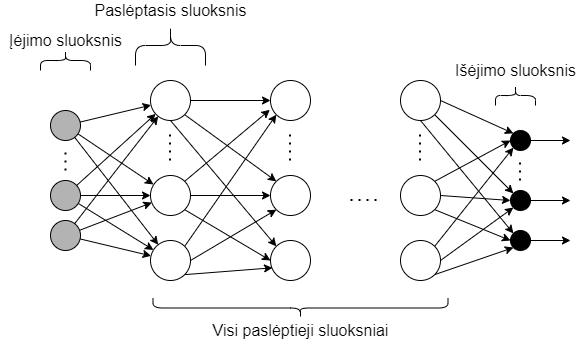
\includegraphics[scale=0.5]{img/neural_network.png}
	\caption{Daugiasluoksnis perceptronas}
	\label{img:nn}
\end{figure}

Daugiasluoksnis perceptronas pateiktam vektoriui $\boldsymbol{x}'$ priskiria klasę, kuri buvo priskirta išėjimo sluoksnio perceptronui, kurio išėjimo reikšmė buvo didžiausia iš visų išėjimo sluoksnio perceptronų.

Tam kad daugiasluoksnis perceptronas galėtų atlikti klasifikavimą, jis turi būti apmokytas. Kaip ir perceptronas, daugiasluoksnis perceptronas yra apmokomas iteratyviai keičiant visų perceptronų svorius naudojant formulę (\ref{eqn:w_recalc}). Išėjimo sluoksnio perceptronams yra naudojama bendra formulė (\ref{eqn:general}). Tačiau ši funkcija, paslėptųjų sluoksnių perceptronų mokymui, yra nenaudojama, nes nėra apibrėžta nuostolių funkcija $e(w)$, mat funkcijai $e(w)$ yra reikalingi perceptronų išėjimai, kurie yra nežinomi. Tad paslėptųjų perceptronų svoriai yra keičiami naudojant klaidos sklidimo atgal algoritmą (angl. back-propagation learning algorithm).

Klaidos sklidimo atgal algoritmas yra gradientinio nusileidimo strategijos realizacija daugiasluoksniam perceptronui. Šio algoritmo veikimo santrauka: randamas \textit{i}-tosios iteracijos išėjimo vektorius $Y_i = (y_{i1}, y_{i2}, ..., y_{id})$, apskaičiuojama \textit{i}-tosios iteracijos išėjimo sluoksnio perceptronų paklaidos $e_i(w)$, apskaičiuojami paslėptųjų sluoksnių perceptronų paklaidos, kiekvienam sluoksniui naudojant jo tolimesnių sluoksnių perceptronų paklaidas, ir pakeičiant svorius naudojantis gautomis paklaidomis.

Išėjimo perceptronų paklaidos randamos naudojant formulę (\ref{eqn:mse}). Tad bendru atveju išėjimo sluoksnių svoriai yra keičiami naudojant formulę (\ref{eqn:general}). Įvedamas lokalaus gradiento žymėjimas (\ref{eqn:loc_grad}), kur $y_{ij}$ yra gauta išėjimo reikšmė, $t_{ij}$ - norima išėjimo reikšmė su \textit{i}-tuoju įėjimo vektoriumi \textit{j}-tajam perceptronui, $a_{ij}$ apskaičiuojamas pagal lygtį (\ref{eqn:activ_arg}) naudojant \textit{j}-tojo perceptrono svorius ir \textit{i}-tąjį įėjimo vektorių ir f - aktyvacijos funkcija. Įsistačius šį žymėjimą į formulę (\ref{eqn:general}) gaunama funkcija (\ref{eqn:general_with_loc_grad}).

\begin{equation}
\label{eqn:loc_grad}
	\xi^j_i = (y_{ij} - t_{ij})(f'(a_{ij})
\end{equation}

\begin{equation}
\label{eqn:general_with_loc_grad}
	w_j(t + 1) = w_j(t) - \eta \dfrac{2}{n}\sum_{i = 1}^{n} \xi^j_i(\sum_{k = 0}^{p} x_{ik}))
\end{equation}

Remiantis darbu \cite{feedbackAlg}, lokalus gradientas $\xi^j$ yra apskaičiuojamas pagal formulę (\ref{eqn:loc_grad_calc}), kur $P_j$ yra aibė perceptronų, prijungtų prie \textit{j}-tojo perceptrono išėjimo, $w_{bj}$ - \textit{b}-tojo ir \textit{j}-tojo perceptronų jungties svoris.

\begin{equation}
\label{eqn:loc_grad_calc}
	\xi^j_i = f'(a_{ij})\sum_{b \in P_j}\xi^b_i w_{bj}
\end{equation}

Tad bendru atveju daugiasluoksnio perceptrono svoriai yra keičiami naudojantis formule (\ref{eqn:general_mlp}).

\begin{equation}
\label{eqn:general_mlp}
w_j(t + 1) = w_j(t) - \eta \dfrac{2}{n}\sum_{i = 1}^{n} (f'(a_{ij})(\sum_{b \in P_j}\xi^b_i w_{bj})(\sum_{k = 0}^{p} x_{ik}))
\end{equation}

Egzistuoja įvairūs metodai naudojami pradinių svorių parinkimui. Tačiau analizuoto šaltinio \cite{initNN} tyrimai neįrodė, kad vienas iš jų būtų pranašesnis už kitus. Todėl šio magistro baigiamojo darbo tyrimams pradiniai svoriai yra parenkami atsitiktinai.

Procesas, kurio metu yra įvykdomas klaidos sklidimo atgal algoritmas su kiekvienu įėjimo vektoriumi iš mokymo duomenų aibės po vieną kartą, yra vadinamas epocha. Daugiasluoksnio perceptrono apmokymas gali būti vykdomas nurodytą kiekį epochų arba perceptrono apmokymo epochos gali būti vykdomos tol kol nepasiekiamas norimas tikslumas naudojantis validacijos duomenimis. Šiame magistro baigiamajame darbe dirbtinių neuroninių tinklų palyginimui yra naudojami tik apmokymo laiko ir tikslumo kriterijai. Tad tyrime vykdomų epochų skaičiai yra konstantos. Naudojant tą patį epochų skaičių dviems skirtingiems dirbtiniams neuroniniams tinklams, dėl skirtingos tinklų struktūros, apmokymo epochos laikas skiriasi. Tad nurodant tą patį kiekį epochų skirtinguose dirbtinių neuroninių tinklų apmokymuose galima palyginti jų tikslumą ir apmokymo laiką.

Su kiekviena epocha dirbtinis neuroninis tinklas vis tiksliau klasifikuoja apmokymo duomenų vektorius. Tačiau apmokymo duomenys tėra tik poaibis realaus pasaulio duomenų, vadinamų populiacija. Apmokymo duomenys niekada nėra pilnai reprezentatyvūs populiacijai. Todėl po tam tikro skaičiaus epochų, dirbtinio neuroninio tinklo tikslumas priskiriant populiacijos vektorius, kurie nepriklauso apmokymo duomenims, ima mažėti. Ši problema yra vadinama persimokymu (angl. overfitting). Tad dirbtinio neuroninio tinklo tikslumo, kuris būtų reprezentatyvus populiacijai, nustatymui, yra taikomi įvairūs metodai. Du populiariausi šių metodų pavyzdžiai yra f-dalių kryžminis validavimas (angl. f-folds cross validation) ir validavimas su testiniais duomenimis. Šiame magistro baigiamajame darbe naudojamas metodas yra validavimas su testiniais duomenimis, nes šiuo metodu apskaičiuotų dviejų dirbtinių neuroninių tinklų tikslumų palyginimas yra lengviau interpretuojamas.

Apmokytų dirbtinių neuroninių tinklų tikslumo nustatymui, naudojant validavimą su testiniais duomenimis, turimų duomenų aibė yra padalinama į du poaibius: apmokymo duomenis ir testavimo duomenis.  Apmokymo duomenys yra naudojami tik apmokymo procesui. Tuo metu testavimo duomenys yra naudojami apskaičiuoti tikslumui. Šių duomenų vektoriams apmokyti dirbtiniai neuroniniai tinklai priskiria po klasę, kuri yra palyginama su tikrąja vektoriaus klase. Tada apskaičiuojamas tikslumas, naudojantis formule $acc = \dfrac{m}{n}$, kur $m$ yra skaičius vektorių, kuriems priskirta klasė sutapo su jų tikrąja klase ir $n$ - testavimo duomenų vektorių kiekis.
